\subsubsection{Mirai Botnet}
\label{sec:mirai}

The Mirai botnet, composed primarily of embedded and IoT devices, took
the Internet by storm in late 2016 and conducted several DDoS attacks
against Krebs on Security, OVH, and Dyn. Mirai spreads by conducting
random IP scans through TCP SYN probes, which mainly target Telnet TCP
ports 23 and 2323. Once Mirai identifies a potential victim, it
attempts to brute-force log into Telnet. As a result, the Mirai botnet
generates scanning and brute-force traffic during its propagation, and
presumably our scan and brute-force feeds should capture some of this
traffic. We use the data collected by Z.\ Ma et
al.~\cite{antonakakis2017understanding} to measure this overlap.  More
specifically, the data consists of daily snapshots of active Mirai
botnet IPs from August 1, 2016 to February 28, 2017, collected using
the Merit Network's Internet telescope.  This time period is later
than most of our sources' time window, so for this analysis we only
compare this data with our threat intel brute-force data during the
same time period.

%\begin{figure}
%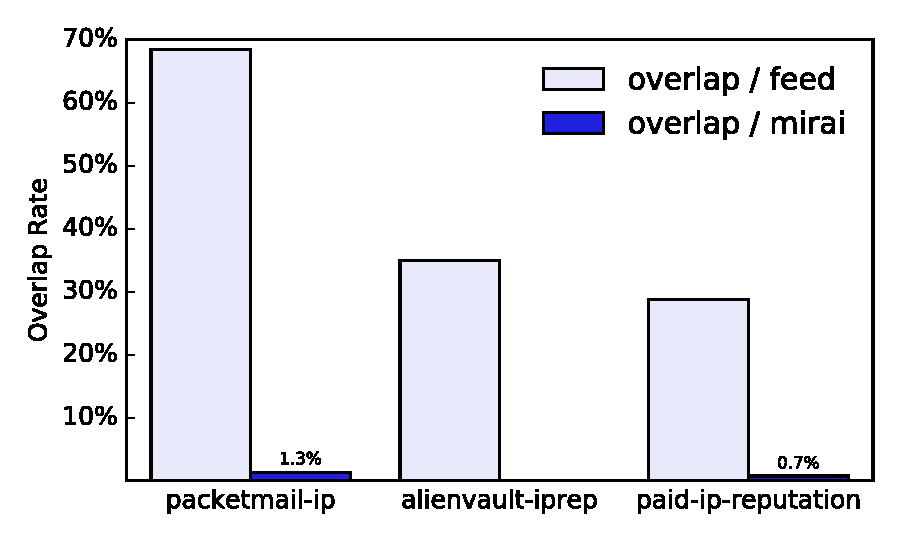
\includegraphics[width=0.95\linewidth]{images/mirai_scan_overall_overlap.pdf}
%\caption{Overall intersection between Mirai botnet and scan feeds}
%\label{fig:mirai_scan_overall_overlap}
%\end{figure}


%\begin{figure}
%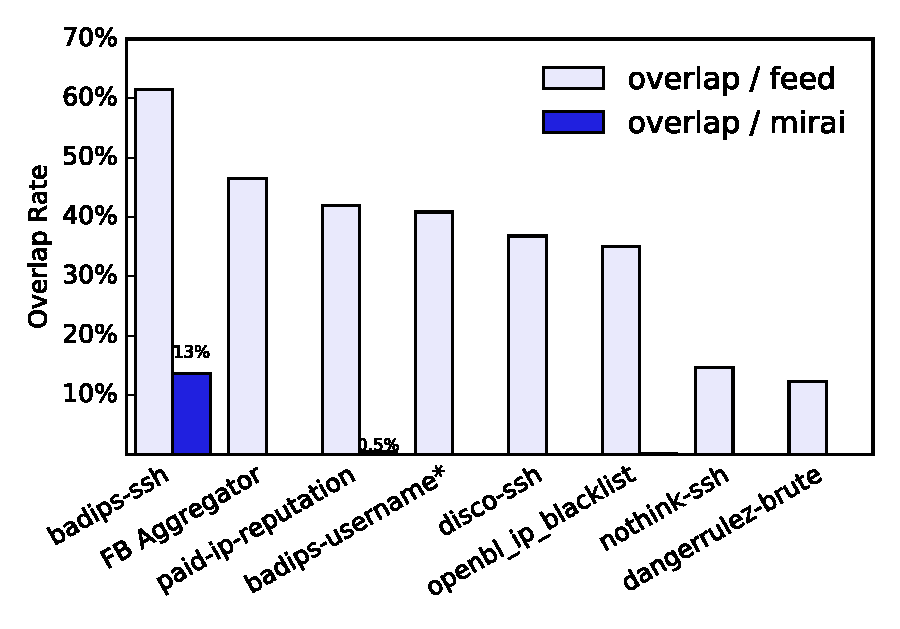
\includegraphics[width=0.95\linewidth]{images/mirai_brute_overall_overlap.pdf}
%\caption{Overall intersection between Mirai botnet and brute-force feeds, light blue bars show the intersection percentage over the feeds' sizes and the dark blue bars %show the percentage over entire Mirai data size. The dark blue bars with no annonatation on the top are less than 0.1\%}
%\label{fig:mirai_brute_overall_overlap}
%s\end{figure}


\begin{table}
\small
\caption{Overall intersection between Mirai botnet and brute-force feeds,
\textit{Inter / Feed} means the intersection percentage over the feeds' sizes.
\textit{Inter / Mirai} shows the coverage percentage over entire Mirai
data size.}
\centering
 \resizebox{0.9\linewidth}{!}{
\begin{tabular}{l r r r}
\toprule
Feed & Volume & Inter / Feed & Inter / Mirai \\
\midrule
{\feedbadipssh}             & 2,801,483    & 61.5\% & 13.68\% \\
%{\feedetiprep}              & 160,205      & 42.0\% & 0.53\% \\
%{\feedopenbl}               & 25,101       & 35.1\% & 0.07\% \\
%{\feeddangerrule}           & 9,365        & 12.4\% & <0.01\% \\
%{\feednothink}              & 7,368        & 14.8\% & <0.01\% \\
%{\feeddisco}                & 3,427        & 37.1\% & 0.01\% \\
%{FB Aggregator}             & 2,975        & 46.5\% & 0.01\% \\
%{Badips Username*}          & 2,564        & 41.0\% & <0.01\% \\
\midrule
%Total & 2,902,735 & 60.0\% & 13.83\% \\
\bottomrule
\end{tabular}
}
\label{tab:mirai_brute_overall_overlap}
\end{table}


There are 12,588,997 unique Mirai IP addresses collected by Merit Network
in the seven-month window. Table~\ref{tab:mirai_brute_overall_overlap} shows
the intersection percentage between the Mirai IP set and each feed. The
feeds not included in the table are the ones we do not have any
data for during the overlapping time period.
Seven out of eight feeds reported less than 1\% of the entire Mirai
dataset. {\feedbadipssh}, however, has over 13\% coverage rate. On the
other side, the Mirai IPs dataset includes a significant amount of the
feeds' data during the time period. Different from scan feeds coverage,
large brute-force feeds like {\feedbadipssh} and {\feedetiprep} also have
relative high coverage of Mirai IPs.

%High /24 aggregations, it means that devices under the same subnet are more likely to be infected, the victims are mainly IoT devices, which could acquire a new IP address under the same after a while.

The Mirai botnet emerged on August 2016 and went through several
phases during its propagation. To better understand how the threat
intel feeds capture these IPs during this seven-month time period, we
measure the intersection between Mirai and the feeds over time, as
shown in Figure~\ref{fig:mirai_brute_daily_overlap}.
%Note that the feeds are in different scale, so for one feed, like {openbl\_ip\_blocklist} 60\% means a few thousands IPs.

%\begin{figure}
%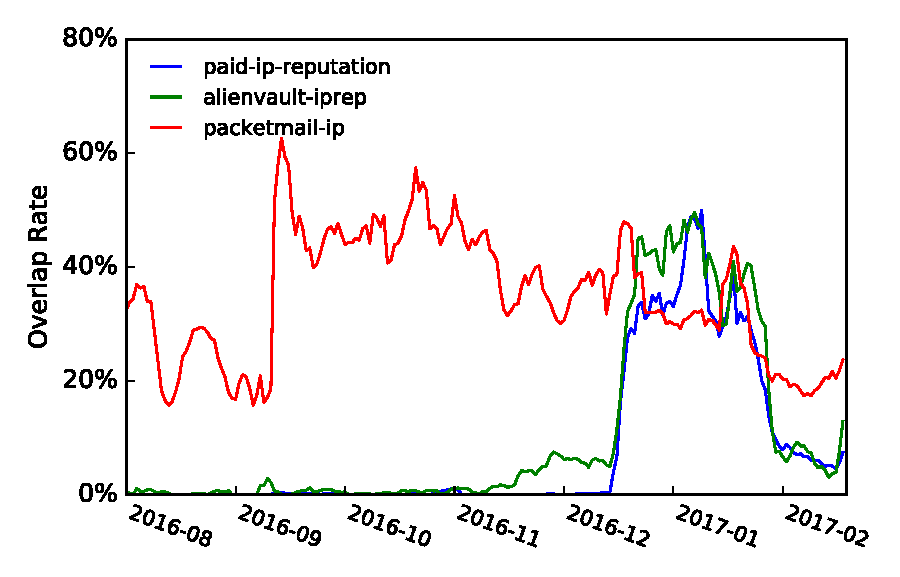
\includegraphics[width=0.95\linewidth]{images/mirai_scan_daily_overlap.pdf}
%\caption{Overlap between Mirai botnet and scan feeds over the time}
%\label{fig:mirai_scan_daily_overlap}
%\end{figure}


\begin{figure}
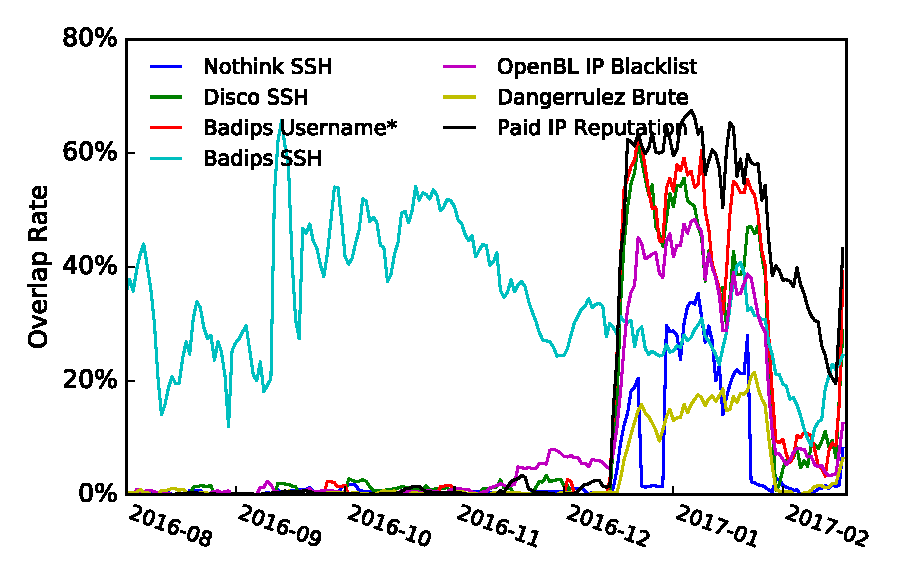
\includegraphics[width=0.95\linewidth]{images/mirai_brute_daily_overlap.pdf}
\caption{Intersection between Mirai botnet and brute-force feeds over the time.
This graph shows that, for each feed, what percent of its data in a 7-day
sliding window consists of Mirai IPs.}
\label{fig:mirai_brute_daily_overlap}
\end{figure}

%More specifically, 6 feeds, except {\feedopenbl},
%have less than 6\% of their data shared with Mirai before December 22nd.
%Between December 22nd, 2016 and Feburary 28th, 2017,

{\feedbadipssh} has a high intersection rate with Mirai across the entire
seven months. For other feeds, as we can see from the graph, reported
few Mirai IPs before December 22, 2016.  Yet, after December 22nd and 23rd,
all these feeds started massively reporting Mirai data.
Figure~\ref{fig:mirai_brute_daily_overlap} shows clear spikes for the feeds
at the same or next day. Diving into the network traffic
initiated by Mirai bots, we observed an emergence of SSH (port 22)
targeted traffic on December 22, 2016, and the source IPs of this
traffic include all the overlapped IPs between the 7 feeds (including {FB Aggregator})
and the Mirai dataset after that time.
Figure 4 in the paper~\cite{antonakakis2017understanding}
also showed this emergence of SSH traffic. This suggests that
these brute-force feeds capture SSH brute-force but mostly do
not cover Telnet (port 23 or port 2323) brute-forcing, which is the primary method
Mirai propagates. {FB Aggregator}, not shown in the graph
for clarity, also has a similar intersection pattern, but the
spike happened over 15 days later and its overlap rate fluctuates
significantly over the time period.

\finding\ The low coverage of these feeds of the Mirai data indicates again
that threat intelligence captured a very limited subset of the IPs
associated with this real-world threat. On the other hand, at their
peak, over 60\% of the data in the feeds are from Mirai, which
demonstrates that the indicators in these feeds contain meaningful
information.


%Another thing worth mentioning is that the spikes in threat intel feeds happened on the same or next day when Merit Network observed a large volume of SSH port scan emerged in the Mirai traffic. This demonstrates that brute-forces feeds can react to a large scale attacks as quick as a large-scale Internet telescope.


%This spike of intersection is easy to understand for brute-force feeds: these brute-force feeds only report SSH brute-force IPs, so they didn't capture the telnet brute-force by most Mirai bots, and start reporting Mirai IPs when this SSH brute-force variant emerged. However, it is surprising that the same thing happened on scan feeds. For a scan feed that reports Internet scanners, one would expect it covers all kinds of port scanning, but from the graph we can tell that scan feeds {\feedetiprep} and {\feedalienvault} don't listen on port 23 or 2323. To verify our conclusion, we go back to the UCSD telescope data we used in the previous section, pick out the scanning traffic that only scanned port 23 or 2323 and see whether they intersection with these two feeds. From the large scanner dataset where source IPs have scanned over 250K IPs in the telescope, we filtered out 1,310 source IPs that only scanned port 23 or 2323, and there are only 6 IPs that overlapped with {\feedetiprep} and 8 IPs that overlapped with {\feedalienvault}, meanwhile, there are 340 IPs that overlapped with {\feedpacketmail}. This validated our conclusion. \note{we might need to move this analysis to the caida case study}
